\documentclass[11pt]{article}
\usepackage[margin=1.0in]{geometry}
\usepackage{ragged2e}
\usepackage{amsmath}    % Expanded math operations for papers
\usepackage{amssymb}
%\usepackage{esvect}    % Vector notation for mathematics
\usepackage{graphicx}
\usepackage{wrapfig}    % Format figures more appropriately
\usepackage{hyperref}   % Enable hyperlink support
\usepackage{fancyhdr}   % Allow headers and footers customized
\usepackage{titlesec}   % Allow customization of section headers
\usepackage{wrapfig}    % So I can wrap figures around my text
\usepackage{enumitem}	% Align things in the itemize environment
%\usepackage{subcaption}
\usepackage{subfig}
\usepackage[font=small,skip=0pt]{caption}

% Set up code environment
\usepackage{listings}
\usepackage{color}

\definecolor{mygreen}{RGB}{28,172,0} % color values Red, Green, Blue
\definecolor{mylilas}{RGB}{170,55,241}

\lstset{language=Matlab,%
    %basicstyle=\color{red},
    breaklines=true,%
    morekeywords={matlab2tikz},
    keywordstyle=\color{blue},%
    morekeywords=[2]{1}, keywordstyle=[2]{\color{black}},
    identifierstyle=\color{black},%
    stringstyle=\color{mylilas},
    commentstyle=\color{mygreen},%
    showstringspaces=false,%without this there will be a symbol in the places where there is a space
    numbers=left,%
    numberstyle={\tiny \color{black}},% size of the numbers
    numbersep=9pt, % this defines how far the numbers are from the text
    emph=[1]{for,end,break},emphstyle=[1]\color{red}, %some words to emphasise
    %emph=[2]{word1,word2}, emphstyle=[2]{style},    
}

% Set graphics path
\graphicspath{ {figures/} }

% Reformat section headers
\titleformat{\section}{\normalfont\large\bfseries}{\thesection}{1em}{}[{\titlerule[0.8pt]}]
\titleformat{\subsection}{\normalfont\large\bfseries}{\thesubsection}{1em}{}
\titleformat{\subsubsection}{\normalfont\normalsize\bfseries}{\thesubsubsection}{1em}{}

% Define page header and footer
\pagestyle{fancy}
\fancyhf{}
\lhead{Seaborn • Buchanan • Sambolu}
\rhead{Mat 7, 2019}
\lfoot{ECE 460}
\rfoot{Page \thepage}

% Define paragraph spacing
\newcommand{\parSpace}{\vspace{0.5cm}}

% Overwrite Subitemize symbol
\renewcommand{\labelitemii}{$\circ$}


\begin{document}



%
%%---------------------------------------------------------------------------------------------------| TITLE
%

\begin{Large}\begin{center}
Music Identification
\end{center}\end{Large}


%
%%---------------------------------------------------------------------------------------------------| PROJECT APPROACH
%

\section{Project Approach}

Our challenge was to replicate the Shazam music detection algorithm proposed by Avery Wang. Reading Wang's paper, \textit{An Industrial-Strength Audio Search Algorithm}, we realized that an identical approach using hashing and constellation analysis would be tedious and besides the point of the project. Rather, our goal is to learn how Fourier series analysis can be applied to real world problems such as audio analysis. We developed a system where a \textit{.WAV} file can be converted into a constellation (fingerprint) of dominant frequency points across time and then compared to new inputs through correlative analysis. This approach requires time to create the database of initial fingerprints but has very little performance overhead to analyze new files once the database has been completed.


%
%%---------------------------------------------------------------------------------------------------| PROCESS
%

\section{Creating Fingerprints}

The creation of finger prints to uniquely represent a music file was the most crucial step in the analysis process. Using the \textit{TwinPeaks.m} function from a previous lab, we adapted our code to find not two but any number of dominant peaks in a given sample. Then we generated a windowing system around the peaks locator which scanned the input song and recorded the dominant frequencies in each time period. The fingerprints are automatically saved for analysis and we have included several of them in Figure ~\ref{Fingerprints}.

We developed these functions to be highly configurable, allowing the technician to determine how many peaks they wanted to save per time period and how many time periods in a song they were willing to save. However these settings must be kept constant lest the comparisons be knocked off track.


\section{Comparing Fingerprints}

With a database of song fingerprints at our disposal, our next task was to compare them to identify new inputs in relation to our database. There were many methods available to us for this task, including the constellation approach detailed by Wang, but we elected to run a correlative analysis with additional windowing of the fingerprint files, see Figure ~\ref{Flow}. In more precise terms, we decided to do the following:

\begin{itemize}[leftmargin = 0.5cm, noitemsep]
	\item \textbf{Create New Fingerprint}
	\begin{itemize}[leftmargin = 1cm, noitemsep]
		\item Take song name as argument
		\item Load \textit{.WAV} file
		\item Get fingerprint values
	\end{itemize}
	\item \textbf{Correlative Analysis}
	\begin{itemize}[leftmargin = 1cm, noitemsep]
		\item Isolate segment of fingerprints
		\item Calculate correlation matrix
		\item Correlation $>=$ Set tolerance
		\begin{itemize}[leftmargin = 1cm, noitemsep]
			\item Return the current song
		\end{itemize}
		\item Correlation $<=$ Set tolerance
		\begin{itemize}[leftmargin = 1cm, noitemsep]
			\item Repeat with next song
		\end{itemize}
	\end{itemize}
\end{itemize}

\begin{figure}[h!]
	\begin{center}
		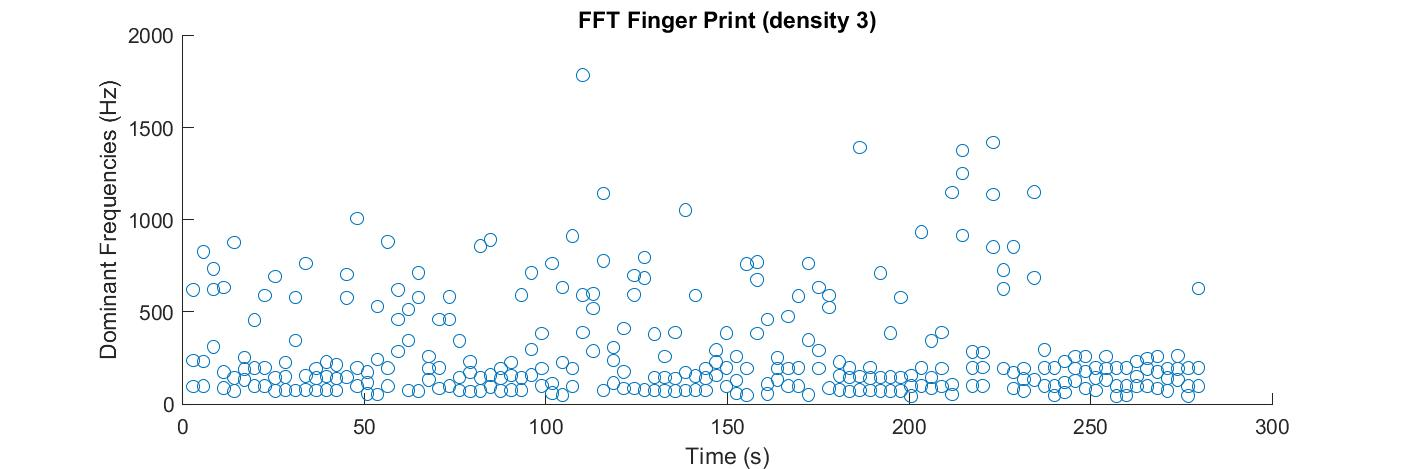
\includegraphics[width=\textwidth]{FingerprintBobMarley.JPEG}
		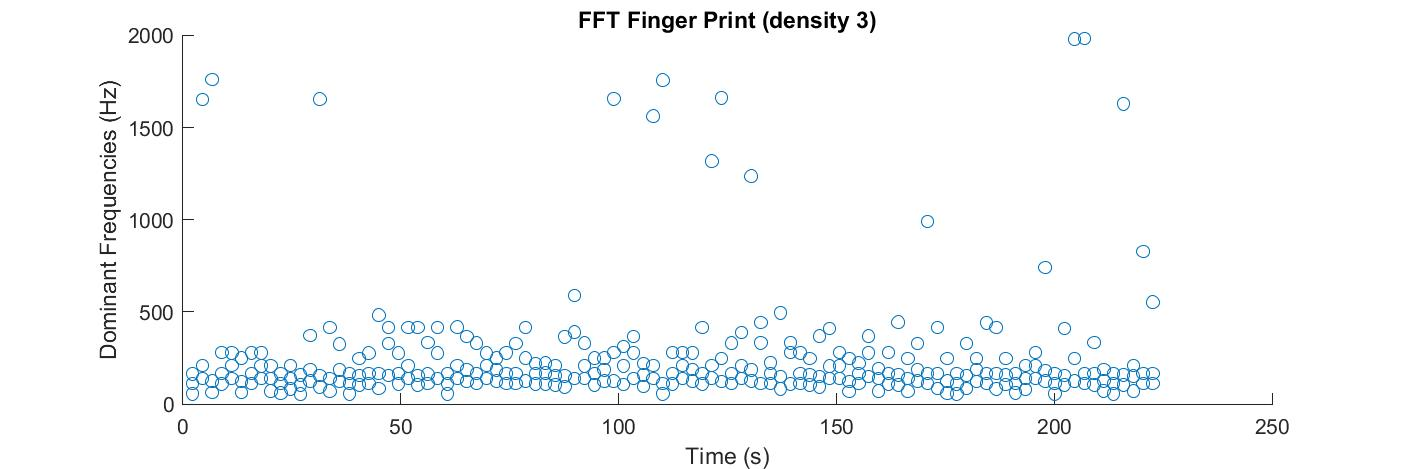
\includegraphics[width=\textwidth]{FingerprintDireStraights.JPEG}
		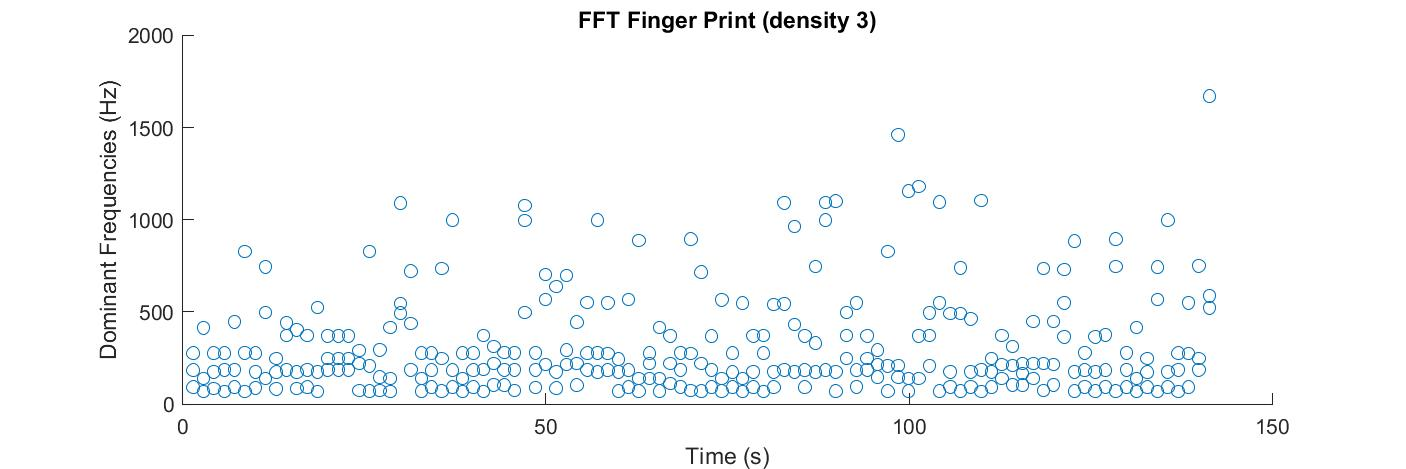
\includegraphics[width=\textwidth]{FingerprintSamCooke.JPEG}
	\end{center}
	\vspace{-1em}
	\caption{ Bob Marley - \textit{I Shot the Sheriff}, \\ Dire Straights - \textit{Lady Writer}, \\ Sam Cooke - \textit{Summertime}. }
	\label{Fingerprints}
\end{figure}


%
%%---------------------------------------------------------------------------------------------------| RESULTS
%

\section{Algorithm Results}

Our system correctly guesses the correct song every time with a 100\% correlation. These results are fantastic and misleading, it only proves that our sampling process does not have stochastic inputs, it is repeatable. In other words, the fact that a 100\% correlation occurs reliably is evidence of the fact that the finger print of the input file and the fingerprint in the database file are identical. This is ideal, our system ought to be stable and our results are testimony to that claim, but there is room for improvement to our existing model. For instance, we could scale the sampling so that there are more samples in the beginning of the time range than at the end, allowing for faster identification of sound files.

We are being too hard on ourselves, the fact remains that this system works perfectly. To test for the robustness against noise, we added a feature to add normalized random values within a specific range to our fingerprints and test if the system fails to detect the signals. Even with aggressive randomness\footnote{We used values between 0 and 200 and achieved $> \: 90 \%$ accuracy.}, our algorithm had no problem identifying the song correctly.

\begin{figure}[h!]
	\begin{center}
		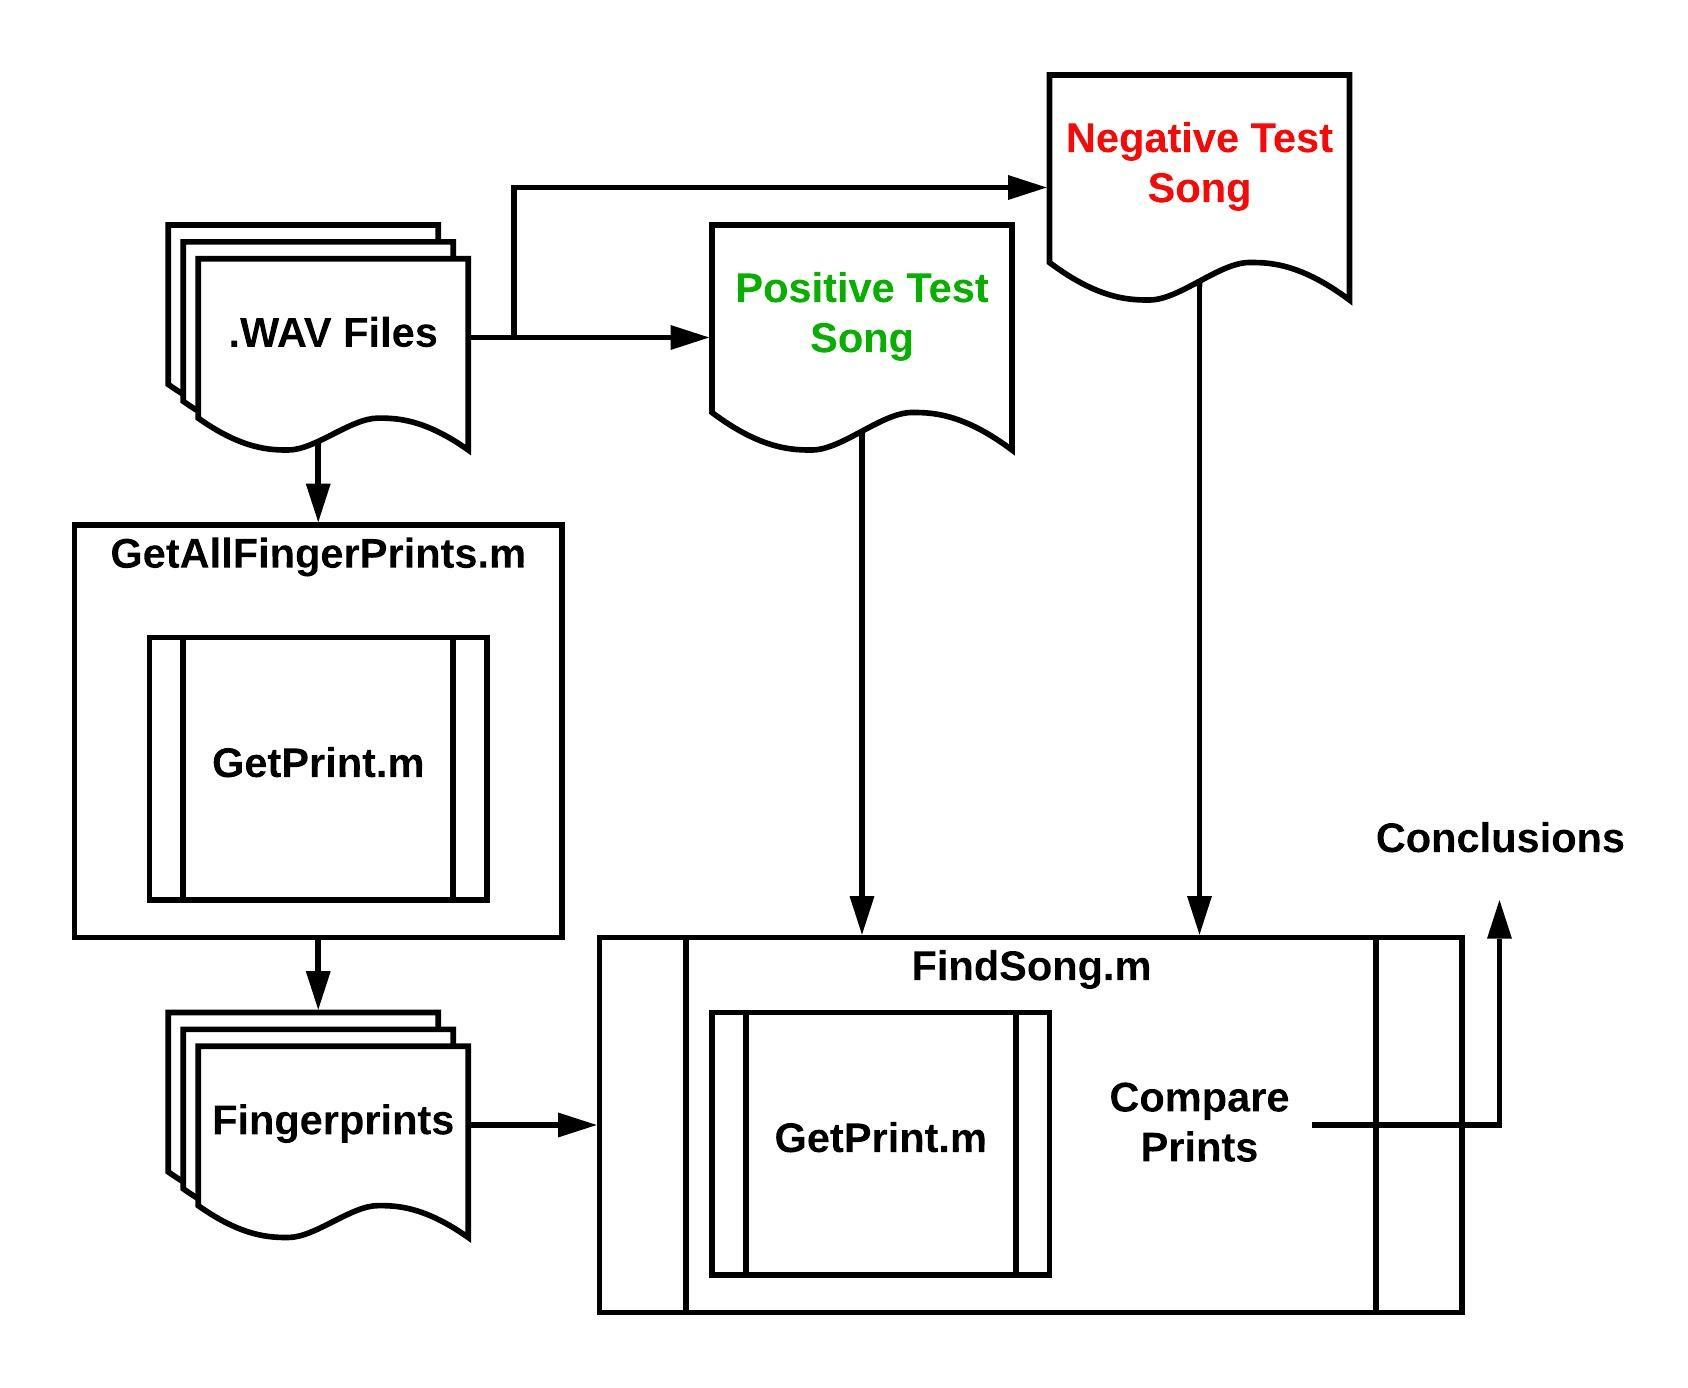
\includegraphics[width=\textwidth]{FlowDiagram.JPEG}
	\end{center}
	\vspace{-1em}
	\caption{ Higher level system architecture. }
	\label{Flow}
\end{figure}



\end{document}

